% !TEX program = xelatex
% !TEX encoding = UTF-8 Unicode
% !TEX spellcheck = de_DE
% 
% © 2015–2017 Moritz Brinkmann, CC-by-sa
% © 2018–2022 Maximilian Jalea, CC-by-sa
% http://latexkurs.github.io

\documentclass[
	vorläufig=false,
	datum=2022-11-16,
	titel={Grafiken, Abbildungen, TikZ},
	web=false,
%	noshortverb=true,
	max,
	aspectratio=1610,
]{../tex/latexkurs-slides}

\usepackage{
	booktabs,
	blindtext,
	siunitx,
	subfloat,
	wrapfig,
	floatflt,
	picinpar,
}


\begin{document}

\begin{frame}{Übersicht}
	\tableofcontents
\end{frame}


\section{Allgemeines}
\begin{frame}{Bilder}
	\begin{block}{Pixelgraphik}
		\begin{itemize}
			\item Menge von Punkten
			\item jedem Punkt wird eine Farbe zugeordnet
			\item Ergebnis von Photos, Scans, etc. 
			\item nicht skalierbar
		\end{itemize}
	\end{block}
	\begin{block}{Vektorgraphik}
		\begin{itemize}
			\item Beschreibung durch mathematische Objekte
			\\ Kurven (Bézier-Kurven, Splines, …) o.\,ä.
			\item beliebig skalierbar
			\item meist kleine Dateigröße
			%\item moderne Schriften sind Vektorgraphiken!
		\end{itemize}
	\end{block}
\end{frame}

\begin{frame}{Bilder in \TeX}
	\begin{itemize}
		\item \TeX\ stammt aus einer Zeit, in der Texte den Informationsaustausch dominierten
		\item \TeX\ kennt \emph{keine} Möglichkeit, externe Bilder einzubinden
		\item \TeX\ kennt nur Boxen
		\item Für alles, was darüber hinaus geht: |\textbackslash special|\pdfmarginpar{Der low-level TeX-Befehl special erlaubt es, beliebige Inhalte direkt in die Ausgabedatei zu schreiben, ohne das TeX sie interpretiert.}
		\item[⇒] abhängig vom „Ausgabegerät“!
	\end{itemize}
\end{frame}

\section{externe Grafiken}
\begin{frame}[fragile]{externe Grafiken}
	\begin{itemize}
		\item \LaTeX\ bietet Möglichkeit, extern erzeugte Bilder einzubinden
		\item je nach Treiber sind verschiedene Formate möglich
		\item u.\,a. jpeg, ps, pdf, gif, tiff, \dots
		\item unter Umständen Umformatierung nötig!
	\end{itemize}
\end{frame}

\begin{frame}{externe Grafiken}
\begin{block}{Vorteile externer Grafiken}
	\begin{itemize}
		\item freie Gestaltungsmöglichkeit
		\item Erzeugung in WYSIWYG-Grafikprogrammen
		\item Unabhängigkeit vom Dokument
		\item spezialisierte Programme für jeden Zweck
		\item einige Programme bieten guten \TeX-Export
	\end{itemize}
\end{block}
\pause
\begin{block}{Nachteile externer Grafiken}
	\begin{itemize}
		\item getrennt vom Dokument ⇒ Portabilität leidet
		\item Layout passt nicht zum Schriftbild
		\item Bildbeschriftungen müssen zur Brotschrift oder Matheschrift passen
		\item Treiberabhängigkeit
	\end{itemize}
\end{block}
\end{frame}

\begin{frame}[fragile]{Inkompatible Formate}
	\begin{itemize}
		\item falls eine Grafik benötigt wird, mit welcher der Treiber nicht umgehen kann:
	\end{itemize}
|\Declaregraphiksrule{|\meta{Endung}|}{|\meta{Typ}|}{|\meta{Größe}|}{|\meta{Befehl}|}|\\
|\DeclareGraphicsRule{.jpg}{eps}{}{'jpg2eps #1'}|
	\begin{itemize}
		\item Paket \pkg{epstopdf} erleichtert Umgang mit PostScript-Dateien
		\item externe Umwandlung empfohlen:\\%
z.\,B. IrfanView, gimp \dots
	\end{itemize}
\end{frame}

\section[graphics/x]{Pakete graphics und graphicx}
\begin{frame}[fragile]{graphics}
	\begin{itemize}
		\item Grundbefehl: |\includegraphics[|\meta{optionen}|]{|\meta{datei}|}|
		\item Dateiendung muss nicht angegeben werden
		\item bei Arbeit mit pdf- \emph{oder} dvi-Ausgabe:
		\item[] Dateiendung besser weglassen
		\item keine absoluten Pfadangaben verwenden (Portabilität)
		\item nützlich, aber nicht ganz zuverlässig: |\graphicspath|
	\end{itemize}
\end{frame}

\begin{frame}[fragile]{graphicx}
	\begin{itemize}
		\item \pkg{graphicx} erweitert \pkg{graphics}
		\item |key=value|-Interface:
		\item[] |[scale = 0.5,angle=50]|
	\end{itemize}
|graphics: \scalebox{0.5}{\includegraphics{a}}|\\
|graphicx: \includegraphics[scale=.5]{a}|
\end{frame}

\begin{frame}[fragile]{Einbinden von Grafiken}
\begin{LTXexample}[pos=b,rframe={}]
\includegraphics[width=2cm]{05_raptor.pdf}
\includegraphics[width=.3\textwidth,angle=25]{05_raptor}
\end{LTXexample}
\end{frame}


\begin{frame}[fragile]{Optionen für \texttt{includegraphics}}
|\includegraphics| kennt viele Optionen, z.\,B.
\\[2ex]
\begin{tabular}{rl}
|scale| & |0.8| \\
|width| & |.2\textwidth|, |15pt|, … \\
|height| & |2em|, |40mm|, … \\
|keepaspectratio| & |true| oder |false|\\
|angle|  & |50| \\
|bb| & |0 0 10 20| \\
|clip| & |true| oder |false|
\end{tabular}
\\[2ex]
⇒ siehe Dokumentation zu \pkg{graphicx}
\end{frame}

\section{interne Grafiken}
\begin{frame}{Bildbeschriftungen}
\begin{description}
\item<+->[Problem] Beschriftungen in externen Grafiken in anderer Schriftart
\item<+->[Lösung] \emph{nackte} Grafik erstellen und Beschriftung mit \TeX\ einfügen\\\LaTeX-Export von z.\,B.  Inkscape nutzen (leider schon lange kaputt)
\item<+->[Lösung] komplette Grafik mit \TeX\ erstellen.
\end{description}
\end{frame}

\subsection{Malen mit \TeX}

\section{Zeichenpakete}
\begin{frame}[fragile]{Zeichenpakete}
	\begin{itemize}
		\item PSTricks – PostScript-Tricks 
		\item \TikZ – \TikZ \emph{i}st \emph{k}ein \emph{Zeichenprogramm}
		\item bieten immens große Möglichkeit, Grafiken zu erstellen
		\item viele spezielle Erweiterungspakete zu PSTricks und \TikZ
		\item z.\,B. Erstellen von Knotendiagrammen, Flussdiagrammen, Schaltplänen etc. 
	\end{itemize}
\end{frame}

\subsection{PSTricks}
\begin{frame}[fragile]{PSTricks}
	\begin{itemize}
		\item Nutzt PostScript-Funktionen um Formen zu erzeugen
		\item funtioniert nicht ohne weiteres mit \hologo{pdfTeX}\\
		|latex|→|dvips|→|ps2pdf| oder \hologo{XeLaTeX} funktionieren
	\end{itemize}
\begin{lstlisting}
\begin{pspicture}(5,5)
  %% rotes Dreieck:
  \psline[linecolor=red](1,1)(5,1)(1,4)(1,1)
  %% grüne Bézierkurve:
  \pscurve[linecolor=green,linewidth=2pt,%
    showpoints=true](5,5)(3,2)(4,4)(2,3)
  %% blauer Kreis mit Radius 1:
  \pscircle[linecolor=blue,linestyle=dashed](3,2.5){1}
\end{pspicture}
\end{lstlisting}
\end{frame}


\subsection{TikZ}
\begin{frame}[t]{\TikZ}
\vfill
	\begin{itemize}
		\item \TikZ ist ein sehr mächtiges Tool
		\item viele Libraries bieten spezialisierte Funktionen:\\
		|arrows|, |automata|, |backgrounds|, |calc|, |calendar|, |chains|, |er|, |intersections|, |mindmap|, …  \pdfmarginpar{Nutzung mittels \ usetikzlibrary\{\}}
		\item viele Pakete bauen auf \TikZ auf bzw. bieten eigene Interfaces:\\
		\pkg{circuitikz}, \pkg{smartdiagram}, \pkg{tikz-dim­line}, \pkg{tikz-palattice}, \pkg{tikz-cd}, \pkg{tikz-inet}, \pkg{hf-tikz}, \pkg{sa-tikz}, \pkg{tikz-bayesnet}, \pkg{tikzposter}, …
		\item Anwendungsbeispiele: \url{http://www.texample.net/tikz/examples/}
	\end{itemize}
\end{frame}


\begin{frame}[fragile,t]{Einfache Objekte in \TikZ}
\begin{description}
	\item<+->[Koordinaten] in runden Klammern: |(|\meta{x-Wert}|,|\meta{y-Wert}|)|\\
		in Standarteinheiten (\si{\centi\meter}):\hfill |(-1,0)|\\
		in belibige Einheiten:\hfill |(5pt,2cm)|\\ 
		in Polarkoordinaten:\hfill |(45:1cm)|\\
		relativ zum vorherigen Punkt:\hfill |+(0,3)|
	\item<+->[Linien]  |\draw[|\meta{Optionen}|] |\meta{Koordinate}| -- |\meta{Koordinate}|;|
\begin{lstlisting}[basicstyle=\ttfamily\scriptsize]
\tikz \draw [red] (0,0) -- (2,0) -- (1,5);
\end{lstlisting}
	\item<+->[Rechtecke] |\draw[|\meta{Optionen}|] |\meta{Koord.}| rectangle |\meta{Koord.}|;|\\[.1ex]
\begin{LTXexample}[pos=r,rframe={},explpreset={basicstyle=\ttfamily\scriptsize},width=2.5cm]
\tikz \draw [fill=blue] (0,0) rectangle (2,0.5);
\end{LTXexample}
	\item<+->[Kreise] |\draw[|\meta{Opt.}|] |\meta{Koord.}| circle [radius=|\meta{Wert}|];|\\[.1ex]
\begin{LTXexample}[pos=r,rframe={},explpreset={basicstyle=\ttfamily\scriptsize},width=2.5cm]
\tikz \draw (0,0) circle
 [x radius=1, y radius =.5];
\end{LTXexample}
\end{description}
\end{frame}

\begin{frame}[fragile]{\TikZ}
\begin{LTXexample}[pos=b]
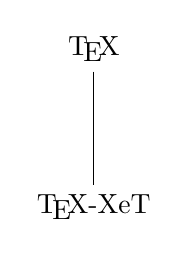
\begin{tikzpicture}
  \node(tex) at (3,2) {\TeX};
  \node(TeX-XeT) at (3,0) {\TeX-XeT};

  \draw(tex) to (TeX-XeT);
\end{tikzpicture}
\end{LTXexample}
\end{frame}



\section{Feinheiten}
\subsection{Teilbilder}
\begin{frame}{Teilbilder}
Besteht eine Abbildung aus mehreren Grafiken, will man diese oft entsprechend zusammenfassen. \vfill
\centering
\includegraphics{05_subcaption}
\end{frame}

\begin{frame}[fragile]{Teilbilder – |subfloat|}
\begin{lstlisting}
\usepackage{subfloat}

\begin{subfigures}
  \begin{figure}
    \centering
    \includegraphics{bild1}
    \caption{Erste Bildunterschrift}
  \end{figure}
  \begin{figure}
    \centering
    \includegraphics{bild2}
    \caption{Zweite Bildunterschrift}
  \end{figure}
\end{subfigures}
\end{lstlisting}
\pkg{subfloat} verändert nur die |figure|-Nummerierung, kann aber keine \emph{gemeinsame} Bildunterschrift erstellen.
\end{frame}



\begin{frame}[fragile]{Teilbilder – |subcaption|}
\begin{lstlisting}
\usepackage{subcaption}

\begin{figure}
  \begin{subfigure}{.5\textwidth}
    \includegraphics{bild1}
    \caption{Erstes Teilbild}
  \end{subfigure}
  \begin{subfigure}{.5\textwidth}
    \includegraphics{bild2}
    \caption{Zweites Teilbild}
  \end{subfigure}
  \caption{Bildunterschrift für beide Bilder}
\end{figure}
\end{lstlisting}

Empfohlene Lösung: \pkg{subcaption}  bietet Umgebung |subfigure| innerhalb von |figure|.
\pdfmarginpar{Im Internet findet man häufig Vorschläge, Teilbilder mit den Paketen subfigure oder subfig zu realisieren. Diese Pakete sind veraltet und inkompatibel mit aktuelleren Paketen wie caption und hyperref.}
\end{frame}


\subsection{textumflossene Grafiken}
\begin{frame}[fragile]{Textumflossene Grafiken}
	\begin{itemize}
		\item aus Textverarbeitungssystemen bekannt:\\%
		Text, der Bild umfließt\\(nicht rechteckig, sondern der Form angepasst)
		\item typographisch fragwürdig – Abhebung des Bildes vom Text
		\item Umfließen stört Lesefluss erheblich
		\item \TeX\ kann prinzipiell keine Graphiken umfließen
		\item mit immensem Aufwand evtl. möglich
		\item Platzierung am Rand einfach möglich
		\item[⇒] Pakete \pkg{wrapfig}, \pkg{picinpar}, \pkg{floatflt}
	\end{itemize}
\end{frame}

\begin{frame}[fragile]{|wrapfig|}
\begin{LTXexample}[preset=\fontsize{4}{5}\selectfont,pos=b]
\blindtext
\begin{wrapfigure}{r}[0.4\width]{0pt}
  \includegraphics[width=2cm]{05_raptor.pdf}
\end{wrapfigure}
\blindtext[3]
\end{LTXexample}
\end{frame}

\begin{frame}[fragile]{|picinpar|}
%syntax: [zeilen bevor, horizontale position, {inhalt des fensters}, {Bildunterschrift}]
\begin{LTXexample}[preset=\fontsize{4}{5}\selectfont,pos=b]
\begin{window}[
  6,c,{\includegraphics[width=2cm]{05_raptor}},{}
]
  \blindtext[4]
\end{window}
\end{LTXexample}
\end{frame}

\begin{frame}[fragile]{|floatflt|}
% floatflt funktioniert super, allerdings nicht mit beamer ;-)
\begin{LTXexample}[preset=\fontsize{4}{5}\selectfont,pos=b]
\blindtext
\begin{floatingfigure}[r]{2cm}
  \includegraphics[width=2cm]{05_raptor}
\end{floatingfigure}
\blindtext[3]
\end{LTXexample}
\end{frame}



\nocite{minimaltikz, tikz, dante:pstricks, graphicscompanion}
\begin{frame}[allowframebreaks]{Weiterführende Literatur}
\printbibliography
\end{frame}

\end{document}
